\documentclass[11pt,a4paper]{article}
\usepackage[utf8]{inputenc}
\usepackage[margin=1in]{geometry}
\usepackage{amsmath}
\usepackage{hyperref}
\usepackage{listings}
\usepackage{xcolor}
\usepackage{tikz}
\usetikzlibrary{shapes,arrows,positioning,decorations.pathreplacing}

\title{Zed's Context Management Architecture: A Transparent Text-First Approach to LLM Context}
\author{Research Paper}
\date{\today}

\begin{document}

\maketitle

\section{Introduction}

Unlike many AI-powered code editors that use hidden embedding systems and vector databases, Zed takes a radically transparent, text-first approach to context management. The language model sees exactly what the user sees in the Agent Panel—there are no opaque vector stores or secret RAG layers. This paper examines how Zed builds, manages, and delivers context to language models through its text-thread architecture, explicit context injection mechanisms, and tool-based automatic context gathering.

\section{The Text-First Philosophy}

Zed's core principle is transparency: everything the LLM receives is visible in the Agent Panel. The context is built from explicit text blocks that users can see, edit, and control. There is no hidden embedding layer that automatically indexes the entire codebase.

\begin{itemize}
    \item \textbf{Text Threads}: The conversation is stored as editable text blocks (System, You, Assistant)
    \item \textbf{Explicit Context}: All context comes from manual inclusion or tool calls
    \item \textbf{No Hidden Memory}: The prompt is the thread—there is no invisible history
    \item \textbf{Editable History}: Users can rewrite any part of the conversation before resending
\end{itemize}

This approach gives users complete control and visibility over what context the model receives, making it easier to debug, optimize, and understand model behavior.

\section{Thread-Based Context Architecture}

Zed's context management centers around the concept of a "text thread"—a specialized document that contains the entire conversation history.

\begin{figure}[htbp]
\centering
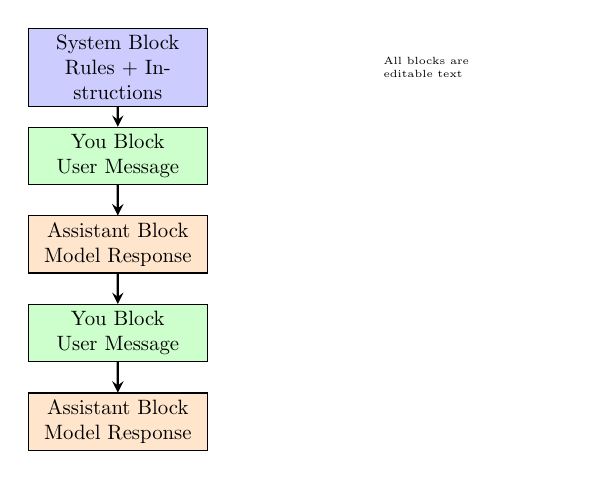
\begin{tikzpicture}[
    node distance=1.5cm,
    box/.style={rectangle, draw, text width=2.8cm, text centered, minimum height=0.8cm},
    system/.style={rectangle, draw, text width=2.8cm, text centered, minimum height=0.8cm, fill=blue!20},
    user/.style={rectangle, draw, text width=2.8cm, text centered, minimum height=0.8cm, fill=green!20},
    assistant/.style={rectangle, draw, text width=2.8cm, text centered, minimum height=0.8cm, fill=orange!20},
    arrow/.style={->, >=stealth, thick},
    scale=0.75,
    transform shape
]
    \node[system] (system) {System Block\\Rules + Instructions};
    \node[user, below of=system] (user1) {You Block\\User Message};
    \node[assistant, below of=user1] (assistant1) {Assistant Block\\Model Response};
    \node[user, below of=assistant1] (user2) {You Block\\User Message};
    \node[assistant, below of=user2] (assistant2) {Assistant Block\\Model Response};

    \draw[arrow] (system) -- (user1);
    \draw[arrow] (user1) -- (assistant1);
    \draw[arrow] (assistant1) -- (user2);
    \draw[arrow] (user2) -- (assistant2);
    
    \node[right of=system, xshift=4.5cm, text width=3cm, font=\tiny] {All blocks are\\editable text};
\end{tikzpicture}
\caption{Text Thread Structure}
\label{fig:thread}
\end{figure}

When a user sends a message, Zed converts these text blocks into a standard chat messages array (system, user, assistant) and sends it to the chosen provider. The thread itself is the prompt—there is no separate "memory" object.

\section{Building Context: Manual Injection Methods}

Zed provides several explicit ways to inject context into a thread. All of these methods result in literal text being inserted into the conversation.

\subsection{Slash Commands}

Slash commands are the primary mechanism for adding context. When executed, they resolve once and paste their results directly into the thread as text.

\begin{itemize}
    \item \texttt{/file <path>} – Inserts file contents or directory tree
    \item \texttt{/tab [name|all]} – Inserts current tab or all open tabs
    \item \texttt{/selection} – Inserts the current text selection
    \item \texttt{/diagnostics} – Inserts language-server diagnostics
    \item \texttt{/terminal [n]} – Inserts last N lines of terminal output
    \item \texttt{/now} – Inserts current date/time
    \item \texttt{/symbols} – Inserts symbol outline of current file
    \item \texttt{/prompt <name>} – Inserts saved rules
    \item \texttt{/fetch <url>} – Fetches content from HTTP endpoint
\end{itemize}

Important: Folds in the UI are just visual—the model still sees all the text. Token counts include folded content.

\subsection{@-Mentions}

The Agent Panel supports @-mentions for adding context:

\begin{itemize}
    \item @files – Mention specific files
    \item @directories – Mention entire directories
    \item @symbols – Mention code symbols
    \item @threads – Reference previous conversations
    \item @rules – Reference saved rule files
\end{itemize}

Mentions are resolved when building the final request, similar to slash commands. They expand into tagged sections within a \texttt{<context>} block, clearly labeled so the LLM knows what was attached by the user.

\begin{figure}[htbp]
\centering
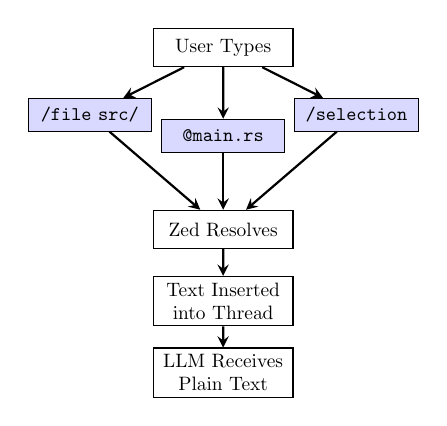
\begin{tikzpicture}[
    node distance=1.3cm,
    box/.style={rectangle, draw, text width=2.3cm, text centered, minimum height=0.7cm},
    command/.style={rectangle, draw, text width=2cm, text centered, minimum height=0.6cm, fill=blue!15},
    arrow/.style={->, >=stealth, thick},
    scale=0.7,
    transform shape
]
    \node[box] (user) {User Types};
    \node[command, below left of=user, xshift=-1.5cm, yshift=-0.3cm] (slash) {\texttt{/file src/}};
    \node[command, below of=user, yshift=-0.3cm] (mention) {\texttt{@main.rs}};
    \node[command, below right of=user, xshift=1.5cm, yshift=-0.3cm] (select) {\texttt{/selection}};
    \node[box, below of=user, yshift=-2cm] (resolve) {Zed Resolves};
    \node[box, below of=resolve] (insert) {Text Inserted\\into Thread};
    \node[box, below of=insert] (llm) {LLM Receives\\Plain Text};

    \draw[arrow] (user) -- (slash);
    \draw[arrow] (user) -- (mention);
    \draw[arrow] (user) -- (select);
    \draw[arrow] (slash) -- (resolve);
    \draw[arrow] (mention) -- (resolve);
    \draw[arrow] (select) -- (resolve);
    \draw[arrow] (resolve) -- (insert);
    \draw[arrow] (insert) -- (llm);
\end{tikzpicture}
\caption{Context Injection Flow}
\label{fig:injection}
\end{figure}

\section{System Prompt Construction}

The system prompt is built from multiple sources and is always prepended to every request.

\subsection{Rules and Project Context}

Zed automatically scans project directories for rule files matching patterns like:
\begin{itemize}
    \item \texttt{.rules}
    \item \texttt{.cursorrules}
    \item \texttt{.windsurfrules}
    \item \texttt{.clinerules}
    \item \texttt{.github/copilot-instructions.md}
    \item \texttt{AGENT*.md}, \texttt{CLAUDE.md}, \texttt{GEMINI.md}
\end{itemize}

These rules are loaded and injected into the system prompt. Additionally, the system prompt includes:
\begin{itemize}
    \item Fixed instructions (communication style, tool usage rules)
    \item List of visible worktree roots
    \item Operating system, architecture, and shell information
    \item Model name and capabilities
    \item User's custom rules from the Rules Library
\end{itemize}

\begin{figure}[htbp]
\centering
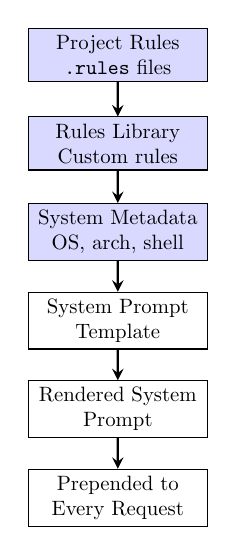
\begin{tikzpicture}[
    node distance=1.5cm,
    box/.style={rectangle, draw, text width=2.8cm, text centered, minimum height=0.8cm},
    source/.style={rectangle, draw, text width=2.8cm, text centered, minimum height=0.7cm, fill=blue!15},
    arrow/.style={->, >=stealth, thick},
    scale=0.75,
    transform shape
]
    \node[source] (rules) {Project Rules\\\texttt{.rules} files};
    \node[source, below of=rules] (library) {Rules Library\\Custom rules};
    \node[source, below of=library] (metadata) {System Metadata\\OS, arch, shell};
    \node[box, below of=metadata] (template) {System Prompt\\Template};
    \node[box, below of=template] (render) {Rendered System\\Prompt};
    \node[box, below of=render] (prepend) {Prepended to\\Every Request};

    \draw[arrow] (rules) -- (library);
    \draw[arrow] (library) -- (metadata);
    \draw[arrow] (metadata) -- (template);
    \draw[arrow] (template) -- (render);
    \draw[arrow] (render) -- (prepend);
\end{tikzpicture}
\caption{System Prompt Construction}
\label{fig:system}
\end{figure}

\section{Automatic Context via Tools}

While manual context injection gives users control, Zed's built-in agent can also automatically gather context through tool calls.

\subsection{Built-in Tools}

Zed's agent has access to tools that allow it to:
\begin{itemize}
    \item Read files from the project
    \item Search the codebase for symbols
    \item Run terminal commands
    \item Edit files (as discussed in the smart edit paper)
    \item List directories
\end{itemize}

When the agent calls a tool, the tool's output is added as a context message in the conversation. The agent can see these results and use them to generate its response.

\subsection{Profiles}

Zed provides different profiles (Write, Ask, Minimal) that control which tools are available:
\begin{itemize}
    \item \textbf{Write}: Full tool access including file editing
    \item \textbf{Ask}: Read-only tools (read files, search, but no edits)
    \item \textbf{Minimal}: No tools, just conversation
\end{itemize}

Users can see which tools are being used during a response in the Agent Panel UI.

\section{External Context via MCP}

The Model Context Protocol (MCP) allows Zed to integrate with external context servers that provide additional data sources.

\subsection{How MCP Works}

MCP servers expose external data such as:
\begin{itemize}
    \item Database schemas (Postgres, PlanetScale)
    \item GitHub repositories and issues
    \item Web search results (Exa Search)
    \item Analytics and telemetry data
\end{itemize}

When a user invokes an MCP command:
\begin{enumerate}
    \item Zed sends a request to the MCP server
    \item The server runs its logic (which may include embeddings/RAG internally)
    \item The server returns text
    \item Zed pastes that text into the thread
\end{enumerate}

\begin{figure}[htbp]
\centering
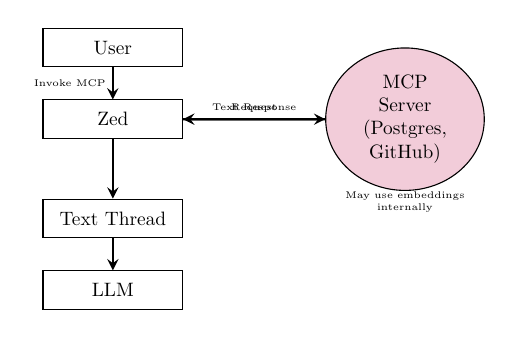
\begin{tikzpicture}[
    node distance=1.3cm,
    box/.style={rectangle, draw, text width=2.3cm, text centered, minimum height=0.7cm},
    server/.style={ellipse, draw, text width=1.8cm, text centered, minimum height=0.9cm, fill=purple!20},
    arrow/.style={->, >=stealth, thick},
    scale=0.7,
    transform shape
]
    \node[box] (user) {User};
    \node[box, below of=user] (zed) {Zed};
    \node[server, right of=zed, xshift=4cm] (mcp) {MCP Server\\(Postgres, GitHub)};
    \node[box, below of=zed, yshift=-0.5cm] (thread) {Text Thread};
    \node[box, below of=thread] (llm) {LLM};

    \draw[arrow] (user) -- node[left, font=\tiny] {Invoke MCP} (zed);
    \draw[arrow] (zed) -- node[above, font=\tiny] {Request} (mcp);
    \draw[arrow] (mcp) -- node[above, font=\tiny] {Text Response} (zed);
    \draw[arrow] (zed) -- (thread);
    \draw[arrow] (thread) -- (llm);
    
    \node[below of=mcp, yshift=-0.2cm, text width=2.2cm, text centered, font=\tiny] {May use embeddings\\internally};
\end{tikzpicture}
\caption{MCP Context Integration}
\label{fig:mcp}
\end{figure}

Key point: Zed itself doesn't manage embeddings. Any vector search happens inside the MCP server, and Zed only receives the final text result.

\section{Session Memory and Summarization}

\subsection{Thread Persistence}

Threads are stored persistently:
\begin{itemize}
    \item All messages (user, assistant, tool calls) are saved
    \item Threads can be reopened from history
    \item Previous threads can be @-mentioned to pull their content into new conversations
\end{itemize}

Storage format: Threads are serialized as JSON or zstd-compressed JSON in \texttt{threads/threads.db}. There is no vector database or embedding index.

\subsection{Token Pressure and Summarization}

Zed tracks token usage and shows a meter in the UI. When approaching the model's context limit:

\begin{enumerate}
    \item Zed suggests starting a new thread
    \item The current thread can be summarized using a separate LLM call
    \item The summary becomes the starting context for the new thread
    \item From that point, the summary text is what persists as "memory"
\end{enumerate}

\begin{figure}[htbp]
\centering
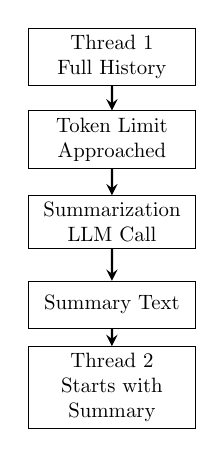
\begin{tikzpicture}[
    node distance=1.4cm,
    box/.style={rectangle, draw, text width=2.6cm, text centered, minimum height=0.8cm},
    arrow/.style={->, >=stealth, thick},
    scale=0.75,
    transform shape
]
    \node[box] (thread1) {Thread 1\\Full History};
    \node[box, below of=thread1] (token) {Token Limit\\Approached};
    \node[box, below of=token] (summarize) {Summarization\\LLM Call};
    \node[box, below of=summarize] (summary) {Summary Text};
    \node[box, below of=summary] (thread2) {Thread 2\\Starts with Summary};

    \draw[arrow] (thread1) -- (token);
    \draw[arrow] (token) -- (summarize);
    \draw[arrow] (summarize) -- (summary);
    \draw[arrow] (summary) -- (thread2);
\end{tikzpicture}
\caption{Thread Summarization Flow}
\label{fig:summarization}
\end{figure}

This is rolling textual summarization, not vector-based retrieval. Long-term memory is implemented as text summaries that users can see and edit.

\section{Complete Context Flow}

Putting it all together, here's how context flows from user input to the LLM:

\begin{figure}[htbp]
\centering
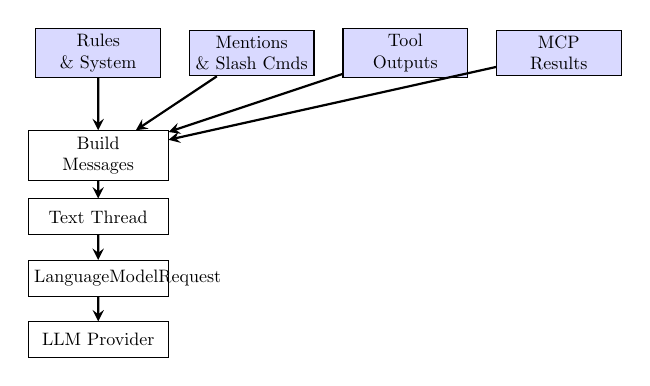
\begin{tikzpicture}[
    node distance=1.2cm,
    box/.style={rectangle, draw, text width=2.5cm, text centered, minimum height=0.7cm},
    source/.style={rectangle, draw, text width=2.2cm, text centered, minimum height=0.6cm, fill=blue!15},
    arrow/.style={->, >=stealth, thick},
    scale=0.65,
    transform shape
]
    \node[source] (rules) {Rules\\\& System};
    \node[source, right of=rules, xshift=1.8cm] (mentions) {Mentions\\\& Slash Cmds};
    \node[source, right of=mentions, xshift=1.8cm] (tools) {Tool\\Outputs};
    \node[source, right of=tools, xshift=1.8cm] (mcp) {MCP\\Results};
    \node[box, below of=rules, yshift=-0.8cm] (build) {Build\\Messages};
    \node[box, below of=build] (thread) {Text Thread};
    \node[box, below of=thread] (request) {LanguageModelRequest};
    \node[box, below of=request] (llm) {LLM Provider};

    \draw[arrow] (rules) -- (build);
    \draw[arrow] (mentions) -- (build);
    \draw[arrow] (tools) -- (build);
    \draw[arrow] (mcp) -- (build);
    \draw[arrow] (build) -- (thread);
    \draw[arrow] (thread) -- (request);
    \draw[arrow] (request) -- (llm);
\end{tikzpicture}
\caption{Complete Context Assembly Pipeline}
\label{fig:complete}
\end{figure}

The final request contains:
\begin{enumerate}
    \item \textbf{System messages}: Built from rules, project context, and system metadata
    \item \textbf{User messages}: Current input plus any retained history
    \item \textbf{Assistant messages}: Previous model responses (if kept)
    \item \textbf{Context blocks}: Resolved mentions, slash commands, tool outputs, MCP results
    \item \textbf{Tool schemas}: Available tools and their definitions
\end{enumerate}

Everything is visible in the Agent Panel—there are no hidden context layers.

\section{Online vs Offline: Context Consistency}

The context building process is identical regardless of whether the model is online or offline:

\begin{itemize}
    \item \textbf{Online (hosted)}: Same text-thread pipeline, full tool support
    \item \textbf{Offline (Ollama/LM Studio)}: Same text-thread pipeline, tools work if model supports them
    \item \textbf{Offline (no tools)}: Same text-thread pipeline, but only explicit context (no automatic tool calls)
\end{itemize}

The difference is in transport and tool capabilities, not in how context is built or stored.

\section{What Zed Does Not Have}

It's important to understand what Zed explicitly does not include:

\begin{itemize}
    \item \textbf{No built-in vector store}: Core Zed does not maintain an embedding index of the codebase
    \item \textbf{No automatic RAG}: There's no hidden retrieval-augmented generation layer
    \item \textbf{No opaque memory}: Everything the LLM sees is visible in the thread
    \item \textbf{No secret context}: No background processes that silently add context
\end{itemize}

If you need vector search or semantic retrieval, you must:
\begin{itemize}
    \item Use an MCP server that implements it (and returns text to Zed)
    \item Build a custom Agent Server that does embeddings internally
    \item Implement it in an external service that Zed calls via MCP
\end{itemize}

\section{Advantages of the Text-First Approach}

Zed's transparent, text-first context management offers several benefits:

\begin{itemize}
    \item \textbf{Debuggability}: Users can see exactly what context the model received
    \item \textbf{Control}: Users decide what context to include, when, and how
    \item \textbf{Predictability}: No hidden behavior that's hard to reason about
    \item \textbf{Editability}: History can be rewritten before resending
    \item \textbf{Composability}: Context sources (rules, files, tools, MCP) are clearly separated
    \item \textbf{Token transparency}: Users can see token usage and optimize accordingly
\end{itemize}

\section{Conclusion}

Zed's context management architecture demonstrates that sophisticated AI assistance doesn't require hidden embedding systems or opaque vector stores. By making context explicit, editable, and visible, Zed gives users the control and transparency needed to effectively work with language models.

The text-first approach means:
\begin{itemize}
    \item Context is built from explicit text inclusion
    \item Everything is visible in the Agent Panel
    \item Memory is stored as editable text threads
    \item Long-term context uses summarization, not vectors
    \item External embeddings (via MCP) are opt-in and transparent
\end{itemize}

This architecture provides a solid foundation for building reliable, debuggable AI-powered development tools while maintaining user control and system transparency.

\end{document}

